\section{Random Variables}

\paragraph{Random variable} A random variable takes numerical values determined by the outcome of a chance process. The \textbf{probability distribution} of a random variable $X$ tells us what the possible values of $X$ are and how probabilities are assigned to those values. There are two types of random variables: discrete and continuous.
\begin{itemize}[font=\sffamily\bfseries, leftmargin=1.95cm, style=nextline, itemsep=0cm]
\item[Discrete] A discrete random variable has a \textit{fixed set of possible values} with gaps between them. The probability distribution assigns each of these values a probability between 0 and 1 such that the sum of all the probabilities is exactly 1. The probability of any event is the sum of the probabilities of all the values that make up the event.
\item[Continuous] A continuous random variable takes all values in some \textit{interval of numbers}. A density curve describes the probability distribution of a continuous random variable. The probability of any event is the area under the curve above the values that make up the event.
\end{itemize}

\paragraph{Expected value} Expected value (a.k.a., \textit{mean}, \textit{expectation}, or \textit{average}) is a weighted average of the possible outcomes of a random variable. Mathematically, if $x_1, x_2, ..., x_n$ are all of the distinct possible values that a discrete random variable $X$ can take, the expected value of $X$ is given by
$$
    \mu_X = \ev[X] = \sum_{i=1}^{n} x_i \pr(X=x_i).
$$

\paragraph{Linearity of expected value} For any random variables $X$ and $Y$, and constants $a$, $b$, and $c$,
$$
    \ev[aX + bY + c] = a\ev[X] + b\ev[Y] + c.
$$

\paragraph{Variance and standard deviation} For a random variable $X$, its variance $\delta_X^2$ is the \textit{average squared deviation} of the values of the variable from their mean; its standard deviation $\delta_X$ is the square root of the variance, measuring the typical distance of the values in the distribution from the mean. For a discrete random variable $X$,
\begin{align*}
    \delta_X^2 &= \var[X] = \sum_{i=1}^{n} (x_i - \mu_X)^2 \pr(X=x_i) \\
    \delta_X   &= \sqrt{\delta_X^2}
\end{align*}

\subsection{Transforming Random Variables}

\paragraph{Addition and subtraction} Adding a positive constant $a$ to (or subtracting $a$ from) a random variable increases (decreases) the mean of the random variable by $a$ but does not affect its standard deviation or the shape of its probability distribution.

\paragraph{Multiplication and division} Multiplying (dividing) a random variable by a positive constant $b$ multiplies (divides) the mean of the random variable by $b$ and the standard deviation by $b$ but does not change the shape of its probability distribution.

\begin{table}[ht!]
    \centering
    \begin{tabular}{cccc}
        \toprule
        & \makecell{Center and location\\\textit{Mean, median,}\\\textit{quartiles, percentiles}}
        & \makecell{Spread\\\textit{range, IQR,}\\\textit{standard deviation}}
        & Shape \\
        \midrule
        $X + a$ & increased by $a$ & No change & No change \\
        $X - a$ & decreased by $a$ & No change & No change \\
        $bX$    & multiplied by $b$ & multiplied by $b$ & No change \\
        $X/b$   & divided by $b$ & divided by $b$ & No change \\
        \bottomrule
    \end{tabular}
\end{table}

\paragraph{Linear transformation} A linear transformation of a random variable involves adding or subtracting a constant $a$, multiplying or dividing by a constant $b$, or both. We can write a linear transformation of the random variable $X$ in the form $Y = a + bX$. The shape, center, and spread of the probability distribution of $Y$ are as follows:
\begin{itemize}[font=\sffamily\bfseries, leftmargin=1.95cm, style=nextline, itemsep=0cm]
\item[Shape] Same as the probability distribution of $X$ if $b > 0$
\item[Center] $\mu_Y = a + b\mu_X$
\item[Spread] $\delta_Y = |b| \delta_X$
\end{itemize}

\subsection{Combining Random Variables}

\paragraph{Mean of combined random variables} If $X$ and $Y$ are \textit{any} two random variables,
$$
    \mu_{X \pm Y} = \mu_X \pm \mu_Y.
$$

\paragraph{Variance of combined random variables} If $X$ and $Y$ are two \textit{independent} random variables,
$$
    \delta^2_{X \pm Y} = \mu_X + \mu_Y.
$$
Note that the variance of either the sum or the difference of two independent variables is \textit{always} the sum of their variances.

\paragraph{Combined normal random variables} Let $X$ and $Y$ be independent random variables that are normally distributed, then their sum is also normally distributed, i.e., if
$$
    X \sim N\left(\mu_X, \delta_X^2\right), \quad
    Y \sim N\left(\mu_Y, \delta_Y^2\right), \quad
    Z = X + Y,
$$
then
$$
    Z \sim N\left(\mu_X + \mu_Y, \delta_X^2 + \delta_Y^2\right)
$$

\subsection{Binomial Distribution}

\paragraph{Binomial coefficient} The binomial coefficient counts the number of ways $k$ successes can be arranged among $n$ trials, calculated by
$$
    {n \choose k} = \dfrac{n!}{k!(n-k)!},
$$
where the factorial of $n$ is
$$
    n! = n(n-1)(n-2) \cdots (3)(2)(1),
$$
for positive whole numbers $n$ and $0! = 1$.

\paragraph{Binomial settings} A binomial setting consists of $n$ independent trails of the same chance process, each resulting in a success or a failure, with probability of success $p$ on each trial. The count $X$ of successes is a \textbf{binomial random variable}. Its probability distribution is a \textbf{binomial distribution}.

\paragraph{Binomial distribution} If $X$ has the binomial distribution with parameters $n$ and $p$, i.e., $X \sim \mathrm{Binomial}(n, p)$, the possible values of $X$ are the whole numbers $0, 1, ..., n$. Its probability mass function (pmf), mean, and variance are given by
\begin{itemize}[font=\sffamily\bfseries, leftmargin=1.95cm, style=nextline, itemsep=0cm]
\item[pmf] $\pr(X=k) = {n \choose k} p^k (1-p)^{n-k}$
\item[Mean] $\mu_X = np$
\item[Variance] $\delta_X^2 = np(1-p)$
\end{itemize}

\paragraph{Shape of binomial distribution} The shape of the binomial distribution is directly controlled by $n$ -- the number of independent trials, and $p$ -- the probability of success.
\begin{itemize}[font=\sffamily\bfseries, leftmargin=3cm, style=nextline, itemsep=0cm]
\item[Small $\mathbf{p}$, small $\mathbf{n}$] The binomial distribution is \textit{skewed right}, i.e., the bulk of the probability falls in the smaller numbers $0, 1, 2, ...$, and the distribution tails off to the right. See Figure \ref{fig:binomial} ($n=15, p=0.1$) and ($n=15, p=0.2$).
\item[Large $\mathbf{p}$, small $\mathbf{n}$] The binomial distribution is \textit{skewed left}, i.e., the bulk of the probability falls in the smaller numbers $n, n-1, n-2, ...$, and the distribution tails off to the left. See Figure \ref{fig:binomial} ($n=15, p=0.8$) and ($n=15, p=0.9$).
\item[$\mathbf{p=0.5}$, all $\mathbf{n}$] The binomial distribution is \textit{symmetric}. See Figure \ref{fig:binomial} ($n=15, p=0.5$) and ($n=40, p=0.5$).
\item[All $\mathbf{p}$, large $\mathbf{n}$] The binomial distribution \textit{approaches symmetry}. For example, if $p=0.2$ and $n$ is small, we'd expect the binomial distribution to be skewed to the right. For large $n$, however, the distribution is \textit{nearly symmetric}. See Figure \ref{fig:binomial} ($n=40, p=0.1$), ($n=40, p=0.2$), ($n=40, p=0.8$), ($n=40, p=0.9$).
\end{itemize}

\begin{figure}[ht!]
    \centering
    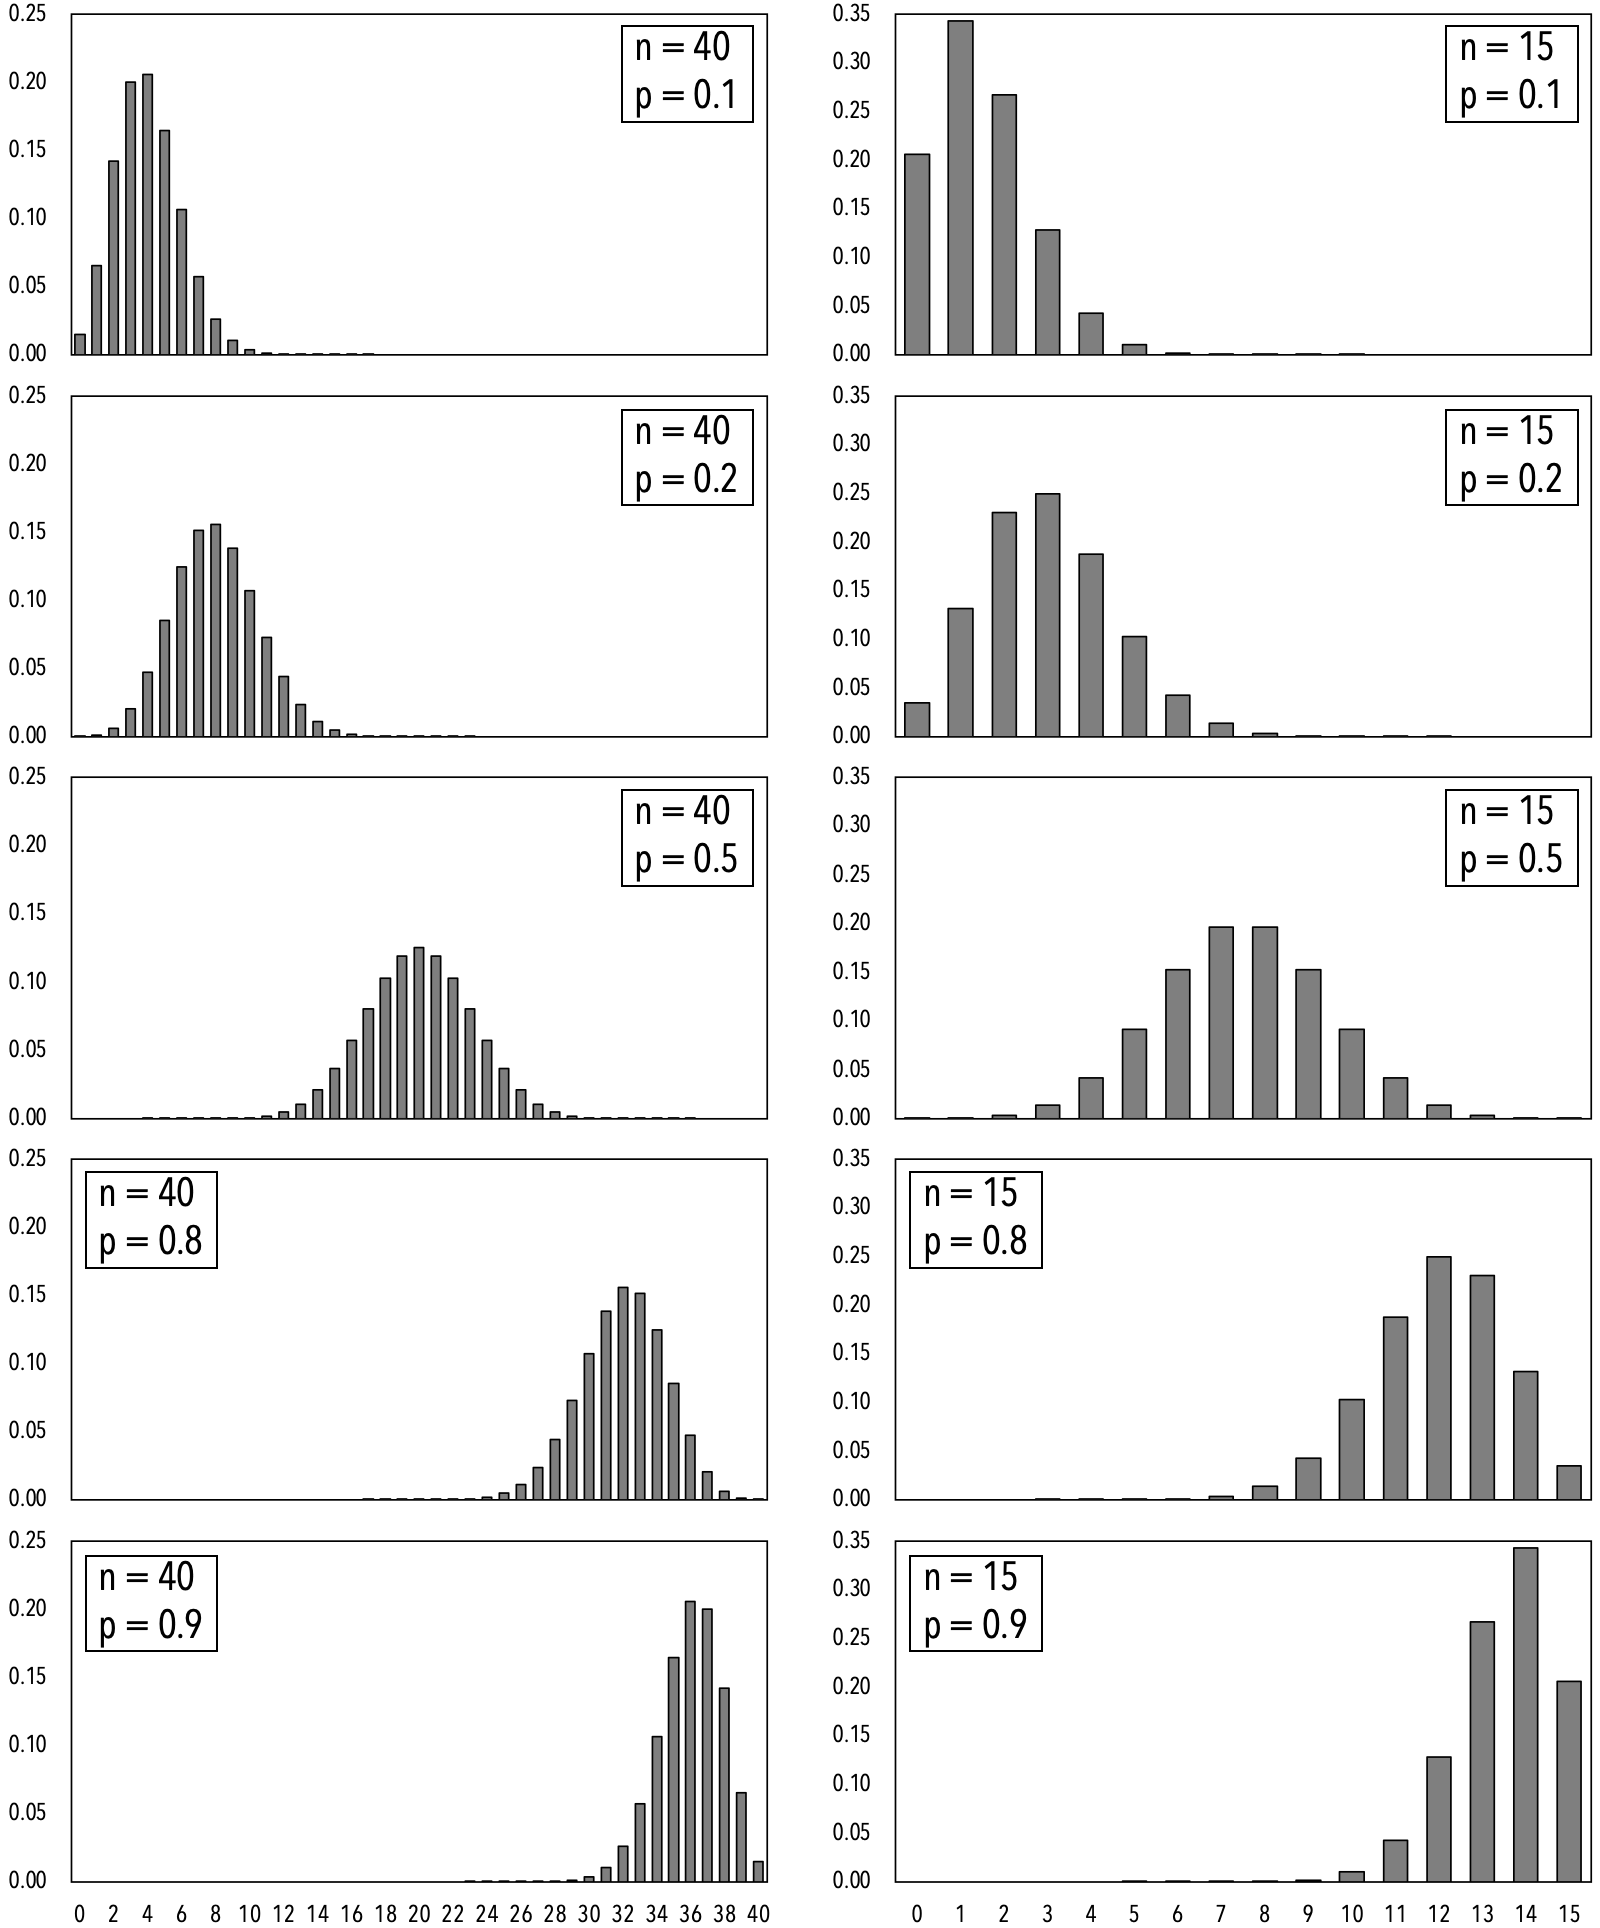
\includegraphics[width=\linewidth]{ch06/binomial.png}
    \caption{Comparison of binomial distribution of different parameters.}
    \label{fig:binomial}
\end{figure}

\subsection{Geometric Distribution}

\paragraph{Geometric settings} A geometric setting consists of repeated trials of the same chance process in which the probability $p$ of success is the same on each trial, and the goal is to count the number of trials it takes to get one success. If $Y$ is the number of trials required to obtain the first success, then $Y$ is a geometric random variable. Its probability distribution is called a geometric distribution.

\paragraph{Geometric distribution} If $Y$ has the geometric distribution with probability of success $p$, i.e., $Y \sim \mathrm{Geometric}(p)$, the possible values of $Y$ are the positive integers $1, 2, 3, ...$. Its probability mass function (pmf), mean, and variance are given by
\begin{itemize}[font=\sffamily\bfseries, leftmargin=1.95cm, style=nextline, itemsep=0cm]
\item[pmf] $\pr(Y=k) = (1-p)^{k-1}p$
\item[Mean] $\mu_Y = 1/p$
\item[Variance] $\delta_Y^2 = (1-p)/p^2$
\end{itemize}

\paragraph{Shape of binomial distribution} The shape of the geometric distribution is directly controlled by $p$ -- the probability of success. The larger the $p$, the steeper the function in the beginning. Note that the function is \textit{monotonically decreasing}.

\begin{figure}[ht!]
    \centering
    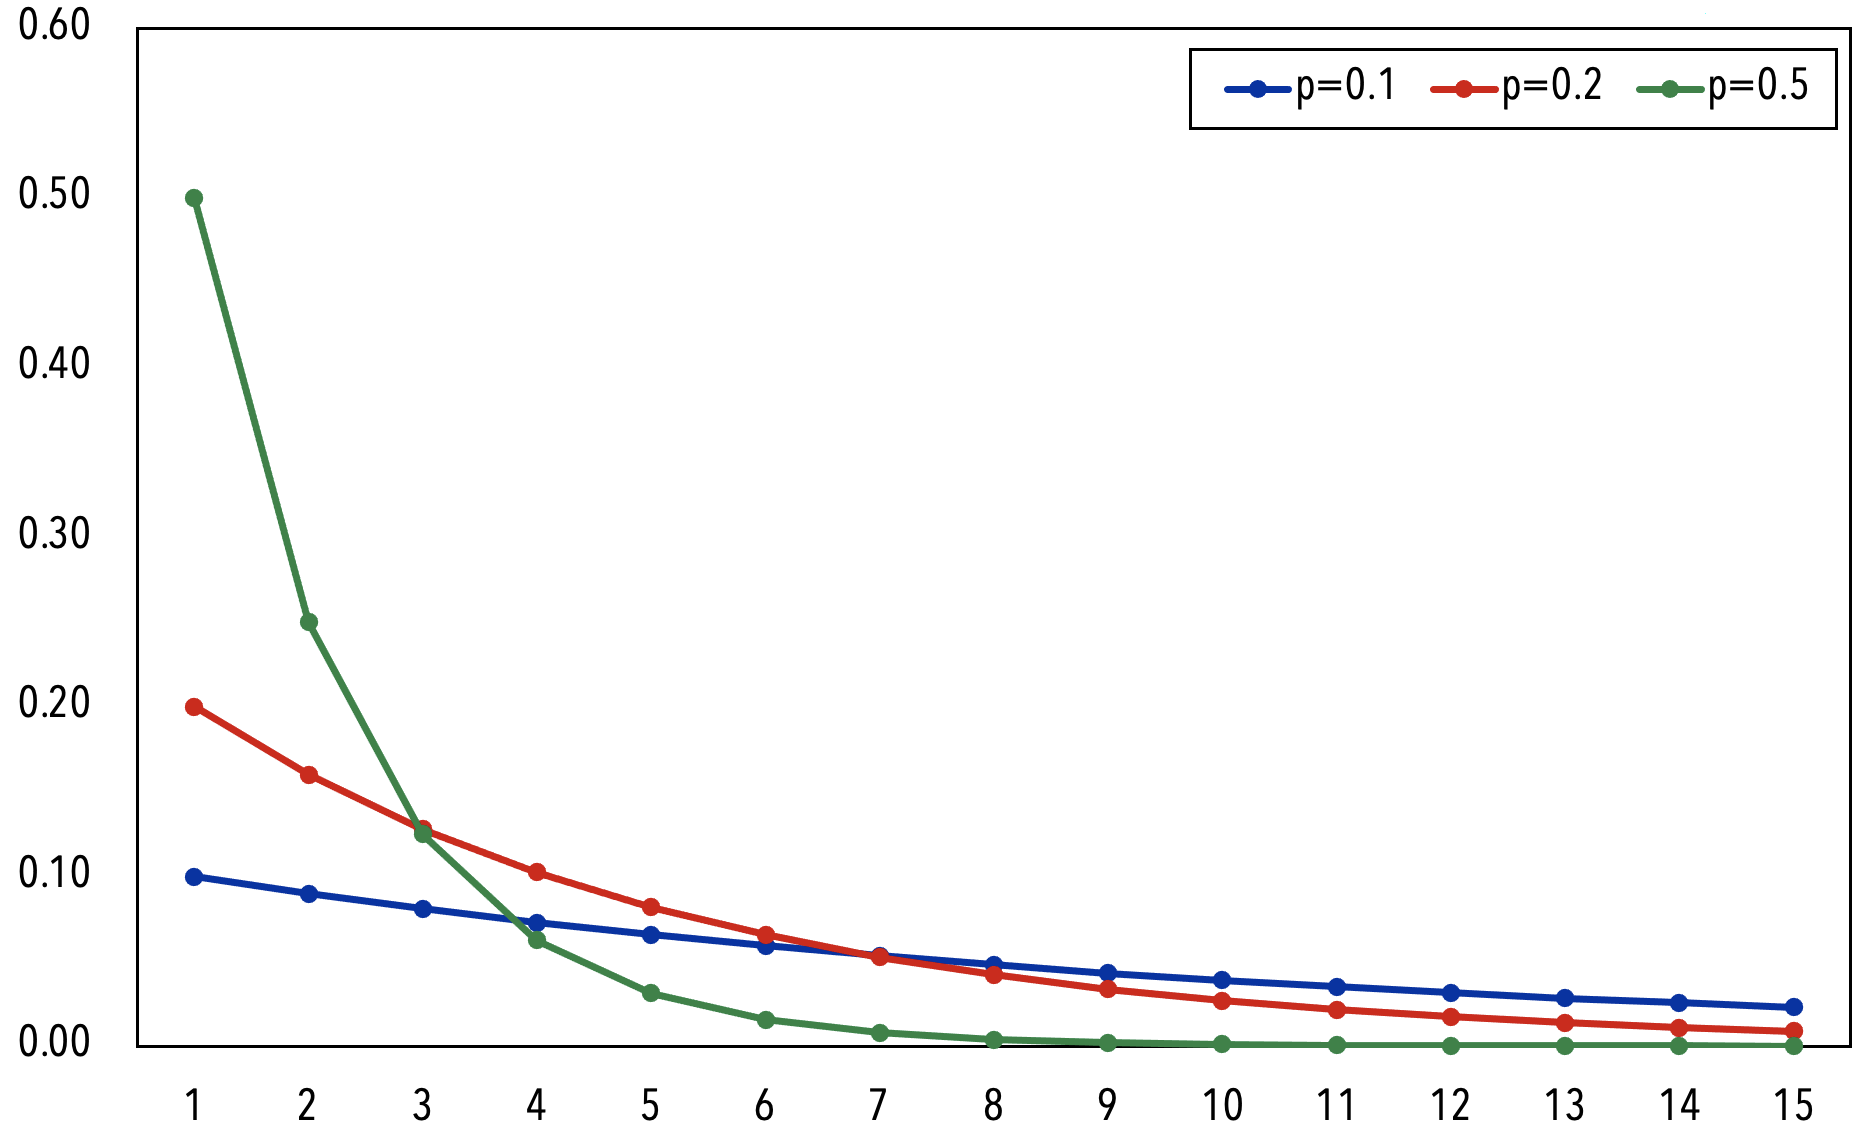
\includegraphics[width=0.8\linewidth]{ch06/geometric.png}
    \caption{Comparison of geometric distribution of different parameters.}
    \label{fig:geometric}
\end{figure}
